\chapter{Estado del Arte}

El estado del arte permite analizar las tendencias, enfoques y limitaciones existentes en la literatura relacionada con la clasificación de residuos de aparatos eléctricos y electrónicos (RAEE), particularmente en el uso de inteligencia artificial, visión computacional y modelos de valoración económica. Este análisis busca identificar los avances más relevantes, así como las brechas de investigación que justifican el desarrollo del presente proyecto.

\section{Preguntas de investigación}

Con el propósito de orientar el análisis de los 58 artículos seleccionados y dar respuesta a las brechas detectadas en la formulación del problema, se establecieron las siguientes preguntas de investigación:

\begin{itemize}
    \item \textbf{P1.} ¿Qué arquitecturas de visión computacional y aprendizaje profundo se han utilizado en los últimos cinco años para la clasificación de residuos electrónicos y qué métricas de desempeño reportan?
    \item \textbf{P2.} ¿Qué características presentan los conjuntos de datos empleados para el entrenamiento y la evaluación de estos modelos en términos de tamaño, número de clases, fuente y nivel de granularidad?
    \item \textbf{P3.} ¿De qué manera se han integrado los modelos de visión computacional con sistemas de apoyo a la toma de decisiones y con esquemas de valoración económica de los RAEE?
    \item \textbf{P4.} ¿Cómo se han abordado los condicionamientos del despliegue real, particularmente los relacionados con dispositivos de borde (\textit{edge AI}), restricciones computacionales y robustez frente a condiciones operativas adversas?
    \item \textbf{P5.} ¿En qué medida los estudios incorporan el contexto latinoamericano y, específicamente, la realidad colombiana en términos normativos, operativos y socio-económicos?
\end{itemize}

\section{Categorías de análisis}

Las categorías de análisis se definieron a partir de los criterios de búsqueda establecidos en la revisión sistemática, con el fin de organizar la literatura de acuerdo con las principales líneas de investigación identificadas en el campo de la clasificación de residuos de aparatos eléctricos y electrónicos (RAEE).

\begin{itemize}
    \item \textbf{Frontera tecnológica:} desarrollo de modelos avanzados de visión computacional y aprendizaje profundo para la clasificación automática de residuos electrónicos.

    \item \textbf{Contexto regional y aplicado:} estudios que abordan la implementación de soluciones tecnológicas en escenarios reales, especialmente en entornos con limitaciones operativas y tecnológicas.

    \item \textbf{Gestión y valoración económica:} investigaciones que integran modelos de inteligencia artificial con sistemas de apoyo a la toma de decisiones y estimación del valor económico de los residuos.

    \item \textbf{Despliegue en hardware de bajo costo:} estudios que implementan y evalúan modelos de visión computacional en plataformas de cómputo asequibles (Raspberry Pi, aceleradores neuronales de bajo consumo y módulos Jetson), con énfasis en latencia, consumo energético y técnicas de optimización como la cuantización.
\end{itemize}

\section{Estrategia de búsqueda y extracción de datos}

La presente revisión sistemática se desarrolló siguiendo la metodología PRISMA (\textit{Preferred Reporting Items for Systematic Reviews and Meta-Analyses}), la cual permite estructurar de manera rigurosa el proceso de identificación, selección y análisis de literatura científica relevante.\\

Para la búsqueda de información se utilizaron bases de datos académicas reconocidas como IEEE Xplore, Scopus y ScienceDirect, con el fin de cubrir la frontera tecnológica en inteligencia artificial y visión computacional. Adicionalmente, se incluyó la base de datos SciELO para incorporar estudios en contexto regional latinoamericano, considerando la limitada disponibilidad de investigaciones aplicadas al sector de gestión de RAEE en esta región.\\

La estrategia de búsqueda se construyó a partir de palabras clave en inglés y español, relacionadas con los ejes temáticos de la investigación, entre ellas:

\begin{multicols}{2}
\begin{itemize}
    \item \textit{E-waste classification}
    \item \textit{Waste classification}
    \item \textit{Computer vision}
    \item \textit{Deep learning}
    \item \textit{Object detection}
    \item \textit{YOLO}
    \item \textit{Convolutional Neural Networks (CNN)}
    \item \textit{Vision Transformers}
    \item \textit{Decision support systems}
    \item \textit{Economic valuation}
    \item \textit{Circular economy}
    \item \textit{RAEE}
    \item \textit{Edge AI}
    \item \textit{Raspberry Pi}
    \item \textit{Low-cost hardware}
    \item \textit{Quantization}
\end{itemize}
\end{multicols}

Estas palabras clave fueron combinadas mediante operadores booleanos (AND, OR) con el fin de ampliar o restringir los resultados de búsqueda según la pertinencia de los estudios identificados.\\

Para sostener el flujo PRISMA con un mínimo de fricción operativa, la gestión de los registros recuperados se apoyó en el software de referencias \textit{Zotero}. Esta herramienta permitió consolidar en una sola biblioteca los artículos provenientes de IEEE Xplore, Scopus, ScienceDirect y SciELO, con la posibilidad de importar los metadatos directamente desde el navegador o a partir del DOI. Su uso resultó decisivo en tres frentes complementarios: la detección y eliminación automática de duplicados antes del cribado por título y resumen; la organización de los estudios mediante colecciones y etiquetas que reflejaron las tres categorías de análisis del proyecto (frontera tecnológica, contexto regional aplicado y gestión y valoración económica); y, finalmente, la generación del archivo BibTeX que sustenta las citas del presente documento. La trazabilidad ofrecida por Zotero también facilitó el registro de notas de lectura por artículo, lo cual fue clave a la hora de extraer las métricas comparativas que se discuten más adelante en este capítulo.\\

En una primera fase de identificación, se recopilaron un total de 312 registros provenientes de las bases de datos consultadas. Posteriormente, se realizó un proceso de cribado en el que se eliminaron artículos duplicados (47) y aquellos que no cumplían con los criterios básicos de relevancia a partir de la lectura de título y resumen (148), obteniendo un conjunto preliminar de 117 estudios.\\

En la fase de elegibilidad, se evaluaron los artículos a partir de la lectura del resumen y del texto completo, aplicando los criterios de inclusión y exclusión definidos previamente. Como resultado, se descartaron 59 trabajos por no presentar validación experimental, no estar relacionados con visión computacional aplicada a residuos o no abordar problemáticas afines a la clasificación o gestión de RAEE.\\

Finalmente, se seleccionó un conjunto de 58 artículos que conforman la base bibliográfica del presente estado del arte, los cuales fueron analizados en profundidad con el objetivo de identificar tendencias, enfoques metodológicos predominantes y brechas de investigación.\\

De manera complementaria, y con el fin de sustentar el despliegue del sistema en hardware de bajo costo, se realizó una búsqueda dirigida con los términos \textit{Edge AI}, \textit{Raspberry Pi}, \textit{low-cost hardware} y \textit{quantization}, restringida a publicaciones de 2022 a 2026. Esta búsqueda incorporó siete estudios adicionales, que se analizan en la cuarta categoría y no modifican los conteos del flujo PRISMA presentado a continuación.\\

El proceso completo de selección de artículos se resume mediante un diagrama PRISMA, el cual permite visualizar de forma estructurada las etapas de identificación, cribado, elegibilidad e inclusión de los estudios considerados.

\begin{figure}[H]
\centering
	\resizebox{\textwidth}{!}{
    % --- Paleta de Colores para Esquema PRISMA (Contraste Optimizado) ---

    % Encabezado ("Bases consultadas") - Azul Acero Medio
    \definecolor{headermainblue}{RGB}{176, 196, 222}
    \definecolor{headerborderblue}{RGB}{70, 130, 180}

    % Proceso Principal (Flujo Central) - Gris Azulado Pálido
    \definecolor{mainblue}{RGB}{240, 244, 248}
    \definecolor{borderblue}{RGB}{176, 190, 197}

    % Exclusiones (Lado Derecho) - Salmón Muy Tenue
    \definecolor{mainred}{RGB}{255, 235, 230}
    \definecolor{borderred}{RGB}{210, 160, 150}

    % Resultado Final (Cuadro Inferior) - Verde Salvia Claro
    \definecolor{maingreen}{RGB}{232, 245, 233}
    \definecolor{bordergreen}{RGB}{129, 199, 132}

    % ---------------------------------------------
		\begin{tikzpicture}[
			% Distancia vertical entre nodos principales
			node distance=1.2cm,
			% Estilo base: Relleno sólido, texto negro, bordes definidos
			basebox/.style={
				rectangle, thick, align=center,
				rounded corners=2pt,
				minimum height=1.3cm,
				font=\small,
				text=black
			},
            blueboxheader/.style={basebox, draw=headerborderblue, fill=headermainblue, text width=7.5cm},
			bluebox/.style={basebox, draw=borderblue, fill=mainblue, text width=7.5cm},
			redbox/.style={basebox, draw=borderred, fill=mainred, text width=6cm},
			greenbox/.style={basebox, draw=bordergreen, fill=maingreen, text width=7.5cm},
			% Flechas
			arrow/.style={-{Stealth[length=3mm, width=2mm]}, thick, draw=black!70}
			]

			% --- Flujo Central ---
			\node[blueboxheader] (bases) {\textbf{Bases Consultadas}\\ \footnotesize IEEE Xplore, Scopus, ScienceDirect, SciELO};

			\node[bluebox, below=of bases] (id) {\textbf{Identificación}\\ Registros encontrados: 312};

			\node[bluebox, below=of id] (cribado) {\textbf{Cribado}\\ Registros sin eliminar: 265};

			\node[bluebox, below=of cribado] (eleg) {\textbf{Elegibilidad}\\ Artículos evaluados: 117};

			\node[greenbox, below=of eleg] (incl) {\textbf{Incluidos}\\ \footnotesize Artículos seleccionados: 58};

			% --- Puntos de control (Coordenadas en el centro exacto entre cajas) ---
			\coordinate (m1) at ($(id.south)!0.5!(cribado.north)$);
			\coordinate (m2) at ($(cribado.south)!0.5!(eleg.north)$);
			\coordinate (m3) at ($(eleg.south)!0.5!(incl.north)$);

			% --- Cajas de Exclusión ---
			\node[redbox, anchor=west] (elim) at ([xshift=4.5cm]m1) {\textbf{Eliminados: 47}\\ \footnotesize Duplicados o no relevantes};

			\node[redbox, anchor=west] (desc) at ([xshift=4.5cm]m2) {\textbf{Descartados: 148}\\ \footnotesize No cumplen criterios (título/resumen)};

			\node[redbox, anchor=west] (excl) at ([xshift=4.5cm]m3) {\textbf{Excluidos: 59}\\ \footnotesize Evaluación a texto completo};

			% --- Conexiones Verticales ---
			\draw[arrow] (bases) -- (id);
			\draw[arrow] (id) -- (cribado);
			\draw[arrow] (cribado) -- (eleg);
			\draw[arrow] (eleg) -- (incl);

			% --- Conexiones Laterales ---
			\draw[arrow] (m1) -- (elim.west);
			\draw[arrow] (m2) -- (desc.west);
			\draw[arrow] (m3) -- (excl.west);

		\end{tikzpicture}
	}
\caption{Esquema PRISMA de selección de artículos.}
\label{fig:esquema_prisma}
\end{figure}


\section{Criterios de elegibilidad}

Los criterios de inclusión y exclusión permiten delimitar de manera rigurosa los estudios considerados en la revisión sistemática, garantizando la calidad, pertinencia y actualidad de la literatura analizada. Estos criterios se definieron en coherencia con el objetivo de la investigación y con los lineamientos de la metodología PRISMA.

\subsection{Criterios de Inclusión}

Se consideraron como criterios de inclusión los siguientes:

\begin{itemize}
    \item Estudios científicos publicados en los últimos cinco años (2022--2026) relacionados con la aplicación de inteligencia artificial, visión computacional y aprendizaje profundo en la clasificación de residuos o reconocimiento de objetos.

    \item Artículos que empleen modelos de \textit{deep learning}, como redes neuronales convolucionales (CNN), arquitecturas tipo YOLO o \textit{Vision Transformers}, aplicados a tareas de clasificación o detección de objetos en imágenes.

    \item Investigaciones que integren técnicas de inteligencia artificial con sistemas de apoyo a la toma de decisiones o enfoques de valoración económica en el contexto de la gestión de residuos o economía circular.

    \item Estudios que presenten resultados experimentales con métricas cuantitativas de desempeño, tales como \textit{accuracy}, \textit{precision}, \textit{recall} o \textit{F1-score}.

    \item Publicaciones disponibles en texto completo, en idioma inglés o español, indexadas en bases de datos académicas reconocidas como IEEE Xplore, Scopus, ScienceDirect y SciELO, esta última considerada para incluir estudios en contexto regional latinoamericano, para lo cual fue necesario incorporar algunos artículos previos al rango definido (desde 2020).

    \item Trabajos que aborden la clasificación de residuos electrónicos (RAEE) o problemáticas similares de clasificación de objetos mediante visión computacional.
\end{itemize}

\subsection{Criterios de Exclusión}

Se excluyeron los estudios que cumplieran con alguna de las siguientes condiciones:

\begin{itemize}
    \item Publicaciones anteriores al año 2022, salvo aquellas referencias estructurales utilizadas como contexto regional.

    \item Artículos que no presenten validación experimental o que carezcan de métricas cuantitativas de evaluación.

    \item Estudios enfocados exclusivamente en datos no visuales (texto, audio o series temporales) sin relación con visión computacional.

    \item Publicaciones disponibles únicamente en formato de resumen (\textit{abstract}) sin acceso al texto completo.

    \item Artículos duplicados o versiones preliminares de estudios ya incluidos en su versión final.

    \item Investigaciones que no tengan relación con clasificación, detección o análisis de residuos electrónicos o problemas equivalentes.

    \item Estudios que utilicen metodologías obsoletas o sin relación con técnicas modernas de inteligencia artificial.
\end{itemize}


\section{Resultados de la búsqueda bibliográfica}

A partir de los artículos seleccionados mediante el proceso PRISMA, se presentan a continuación los principales hallazgos organizados en tres ejes: la distribución de los estudios por fuente y año de publicación, el análisis de los enfoques metodológicos identificados en la literatura y las principales tendencias en el uso de técnicas de inteligencia artificial para la clasificación de residuos de aparatos eléctricos y electrónicos (RAEE).

\subsection{Distribución de los estudios}

De los artículos científicos incluidos en la revisión, las bases de datos IEEE Xplore, Scopus y ScienceDirect concentraron la mayor cantidad de publicaciones, evidenciando su relevancia en la difusión de investigaciones relacionadas con inteligencia artificial y visión computacional. Por su parte, SciELO permitió identificar estudios en contexto regional latinoamericano, aportando una perspectiva aplicada al problema de gestión de residuos electrónicos.

\begin{table}[H]
\centering
\caption{Distribución de artículos seleccionados por base de datos}
\begin{tabular}{lc}
\hline
\textbf{Base de datos} & \textbf{Cantidad de artículos} \\
\hline
ScienceDirect & 23 \\
IEEE Xplore & 21 \\
Scopus & 10 \\
SciELO & 4 \\
\hline
\textbf{Total} & 58 \\
\hline
\end{tabular}
\end{table}

En cuanto a la distribución temporal, los estudios seleccionados corresponden al periodo comprendido entre los años 2022 y 2026, observándose un incremento significativo en el número de publicaciones en los últimos años. Este crecimiento está asociado al auge de técnicas de aprendizaje profundo y modelos avanzados de visión computacional aplicados a la clasificación automática de objetos y residuos.

\begin{table}[H]
\centering
\caption{Distribución de artículos por año de publicación}
\begin{tabular}{lc}
\hline
\textbf{Año} & \textbf{Cantidad de artículos} \\
\hline
2020 & 2 \\
2022 & 2 \\
2023 & 9 \\
2024 & 10 \\
2025 & 22 \\
2026 & 13 \\
\hline
\textbf{Total} & 58 \\
\hline
\end{tabular}
\end{table}

El análisis de la literatura evidencia una tendencia creciente hacia el uso de modelos de aprendizaje profundo, especialmente redes neuronales convolucionales (CNN) y arquitecturas basadas en detección de objetos como YOLO, las cuales han demostrado un alto desempeño en tareas de clasificación visual. Asimismo, se observa una adopción progresiva de modelos más recientes como los \textit{Vision Transformers}, que permiten capturar relaciones espaciales complejas en imágenes \cite{chauhanViT4WasteVisionTransformerBased2025, oiseEViTNetLightweightVision2026, donmez_benchmarking_2025}.\\

Por otro lado, aunque existe una amplia producción científica en clasificación de objetos mediante visión computacional, la aplicación específica en la clasificación de residuos electrónicos (RAEE) sigue siendo limitada, especialmente en contextos regionales. Adicionalmente, se identificó que un número reducido de estudios integra estos modelos con sistemas de apoyo a la toma de decisiones o enfoques de valoración económica, lo que evidencia una oportunidad de investigación en la intersección entre inteligencia artificial y gestión sostenible de residuos.

\section{Análisis de la literatura}

A continuación se presenta la síntesis narrativa de los 58 estudios seleccionados, organizada conforme a las cuatro categorías de análisis y orientada a responder las preguntas de investigación previamente formuladas. La Tabla \ref{tab:matriz_general} resume las características principales de los artículos clasificados como \textit{frontera tecnológica}, mientras que las Tablas \ref{tab:matriz_regional} y \ref{tab:matriz_gestion} sintetizan los aportes en \textit{contexto regional aplicado} y \textit{gestión y valoración económica}, respectivamente. Por último, la Tabla \ref{tab:matriz_edge} recoge los estudios de la búsqueda complementaria sobre despliegue en hardware de bajo costo.

\subsection{Frontera tecnológica: visión computacional y aprendizaje profundo aplicados a la clasificación de residuos}

La revisión sistemática evidencia que la frontera tecnológica para la clasificación automatizada de RAEE está dominada por tres familias de arquitecturas: redes neuronales convolucionales (CNN), detectores de objetos basados en YOLO y, más recientemente, \textit{Vision Transformers}. \cite{jinGarbageDetectionClassification2023} integran MobileNetV2 con un módulo de atención CBAM y una etapa de reducción dimensional por PCA para lograr un \textit{accuracy} de 90{,}7\% sobre el dataset Huawei (14\,683 imágenes), con inferencia ejecutada en una Raspberry Pi 4B en aproximadamente 600\,ms por imagen y un modelo 30{,}1\% más liviano que su versión base. Este resultado consolida a las arquitecturas livianas como una opción viable para despliegues operativos con bajo presupuesto computacional, condición especialmente relevante para el contexto colombiano.\\

En la línea de detectores de objetos, \cite{rajeevAdvancingEwasteClassification2025a} comparan YOLOv5, YOLOv7 y YOLOv8 sobre un dataset propio de 700 imágenes y siete categorías de componentes electrónicos (baterías, capacitores, PCB, sensores IoT, LCD, reguladores y resistores). YOLOv8 obtiene un mAP50 de 82{,}1\%, mAP50--95 de 67{,}8\%, \textit{precision} de 83{,}2\% y \textit{recall} de 70{,}4\%, con una inferencia de aproximadamente 15{,}5\,ms (\(\sim\)65\,FPS). De manera complementaria, \cite{midigudlaComparativeAnalysisDeep2025} amplían el alcance del benchmarking a YOLOv8, EfficientDet y Detectron2 sobre el dataset TACO, encontrando que Detectron2 alcanza el mAP50 más alto (78\%) con una \textit{precision} de 97\%, aunque a un mayor costo computacional, mientras que EfficientDet ofrece un balance favorable (mAP50 70{,}3\%, \textit{precision} 89{,}5\%) cuando los recursos disponibles son limitados.\\

La incorporación de \textit{Vision Transformers} representa la innovación más reciente. \cite{oiseEViTNetLightweightVision2026} proponen E-ViTNet, una arquitectura ViT ligera optimizada con \textit{Oppositional Cat Swarm Optimization} (OCSO) y \textit{Self-Supervised Learning} (SSL) para la clasificación de doce categorías de RAEE, alcanzando un \textit{accuracy} de 99{,}0\%, F1 de 99{,}0\% y AUC-ROC cercano al 100\% a 38\,FPS. Este resultado se complementa con \cite{donmez_benchmarking_2025}, quienes muestran que un ViT base preentrenado supera a ResNet-50 (97{,}62\% vs.\ 90{,}48\%) con sólo 6 épocas de entrenamiento, frente a 30 épocas requeridas por la red convolucional. La consistencia de estos resultados refuerza la pertinencia de incluir arquitecturas basadas en transformadores en el espacio de modelos a evaluar para la clasificación de RAEE, siempre que se cuente con un volumen suficiente de datos o se incorporen estrategias de aprendizaje auto-supervisado.\\

En relación con los condicionamientos del despliegue real, varios trabajos han optado por arquitecturas optimizadas para \textit{edge AI}. \cite{p.sLowPowerEdgeAI2026} desarrollan una arquitectura sobre Raspberry Pi AI HAT con NPU Hailo-8L que combina una CNN cuantizada con fusión multisensorial (peso, inducción electromagnética para detección de metal) y un módulo generativo para reentrenamiento continuo, alcanzando un \textit{accuracy} de 93{,}2\% y una latencia menor a 5\,s con un consumo de 7{,}8\,W. La fusión multisensorial reduce los falsos positivos de 6{,}5\% a 4{,}8\% respecto a una clasificación basada únicamente en visión, demostrando el valor de combinar modalidades cuando la apariencia visual de los componentes es ambigua.\\

Otros estudios refuerzan la importancia de la robustez operativa. \cite{dengVisionbasedDetectionSystem2026a} y \cite{khanLeanAIComputerVisionBasedTool2026} aplican YOLOv8 al dataset CODD (2\,554 imágenes, 10 clases de residuos de construcción y demolición), obteniendo en su mejor variante un mAP50 de 84\% con tiempos de inferencia de 8{,}8\,ms; el segundo trabajo introduce además una capa de principios \textit{Lean} (autonomación, \textit{Poka-Yoke}) que reduce el tiempo de segregación de una tonelada a 55\,minutos. Aunque el dominio inmediato no es RAEE, ambas propuestas son altamente transferibles, en particular el manejo de oclusión, polvo y verificación humana ante baja confianza, condiciones recurrentes en plantas colombianas. \cite{zhouMachineLearningClassification2022} ofrece una línea base inicial de CNN sobre cuatro categorías de RAEE (celulares, baterías, controles remotos, bombillas) con \textit{accuracy} del 93{,}9\%, valor que actúa como umbral mínimo de comparación.\\

Cuando la atención se desplaza a fracciones específicas, los plásticos surgen como un objeto de estudio particular. \cite{bhattaraiAIbasedPlasticWaste2026} sintetizan 112 estudios (2015--2025) y reportan que las CNN logran 87--99\%, los modelos YOLO de 0{,}82 a 0{,}92 mAP, y los \textit{Vision Transformers} cifras superiores al 99\% con datasets suficientemente grandes; señalan, sin embargo, que la integración multisensorial (visión + espectroscopía) está aún subexplotada y que la disponibilidad de \textit{datasets} públicos diversos sigue siendo el principal cuello de botella. La conclusión transversal a este conjunto de trabajos es que la frontera tecnológica del campo está madura para el despliegue operativo de modelos basados en transferencia de aprendizaje, siempre que se disponga de datos representativos y se aborden de manera explícita las restricciones de \textit{edge}.\\

Más allá de los detectores genéricos, varios trabajos recientes se han concentrado en componentes de RAEE específicos y en el cierre del ciclo entre clasificación visual y manipulación física del residuo. \cite{guYOLOMDDAddressingInconsistent2025} introducen YOLO-MDD, una variante orientada al reconocimiento de daños en pantallas móviles bajo condiciones de captura inconsistentes; el aporte más interesante reside en el manejo de objetos a múltiples escalas, una limitación frecuente cuando los \textit{smartphones} se inspeccionan sobre bandas transportadoras o mesas de selección. En la misma línea, \cite{wangImprovedYOLObasedWaste2023} adaptan un detector tipo YOLO a un sistema robótico de pinza incorporando módulos de atención que aceleran la inferencia y mantienen una huella de cómputo razonable para celdas industriales; este trabajo es particularmente relevante porque articula la salida del modelo con la lógica de control del actuador, algo que muchos estudios dejan en un plano puramente algorítmico.\\

Otra línea complementaria es la del puntaje de condición. \cite{menagaIntelligentDeviceCondition2026} combinan YOLO con un clasificador XGBoost para asignar a cada dispositivo un puntaje de estado, con el cual se decide si su destino más sostenible es la redistribución digital, la reparación o el reciclaje; este enfoque resulta cercano al esquema de valoración propuesto en la presente investigación, ya que articula una etapa visual con una etapa de decisión basada en aprendizaje supervisado. \cite{ilievEmbeddedSystemEwaste2023} muestran, por su parte, la viabilidad de embeber un modelo de visión computacional para el reconocimiento de RAEE en hardware de bajo costo, una pieza que se alinea con la realidad operativa de los centros de acopio colombianos, donde la infraestructura no suele ser equiparable a la de un laboratorio de investigación.\\

A nivel aplicado, \cite{madusankaUrbanGreenEWasteDetection2025a} integran YOLOv5 dentro de UrbanGreen, una plataforma orientada al ciudadano que combina detección visual con localización de centros de recolección y orientación pedagógica sobre el riesgo asociado a cada residuo; aunque el énfasis es educativo, la arquitectura de doble capa (modelo de detección + lógica de recomendación) prefigura el tipo de despliegue contemplado en este proyecto. Finalmente, en lo que respecta a la disponibilidad de datos, \cite{vogelgesangMaterialFlowComposition2026} liberan un \textit{dataset} público de imágenes RGB de partículas individuales de RAEE triturado acompañadas de su masa por partícula, una contribución que mitiga parcialmente el reiterado problema de escasez de datos abiertos para entrenar modelos de visión sobre fracciones post-trituración.

\begin{table}[H]
\centering
\caption{Síntesis de los principales estudios de frontera tecnológica analizados.}
\label{tab:matriz_general}
\resizebox{\textwidth}{!}{%
\begin{tabular}{p{3.4cm}p{2.6cm}p{3cm}p{3.5cm}p{4.5cm}}
\hline
\textbf{Estudio} & \textbf{Residuo} & \textbf{Arquitectura} & \textbf{Dataset} & \textbf{Métricas reportadas} \\
\hline
\cite{jinGarbageDetectionClassification2023} & Genérico & MobileNetV2 + CBAM + PCA & Huawei-40 (14\,683 img) & Acc 90{,}7\%; latencia 600\,ms en RPi 4B \\
\cite{midigudlaComparativeAnalysisDeep2025} & Genérico & YOLOv8 / EfficientDet / Detectron2 & TACO (6\,000 img) & Detectron2 mAP50 78\%; P 97\% \\
\cite{rajeevAdvancingEwasteClassification2025a} & RAEE & YOLOv5/v7/v8 & Propio 700 img / 7 clases & YOLOv8 mAP50 82{,}1\%; \textasciitilde65 FPS \\
\cite{donmez_benchmarking_2025} & Reciclables & ViT-base vs ResNet-50 & Propio 689 img / 3 clases & ViT acc 97{,}62\% (6 epochs) \\
\cite{oiseEViTNetLightweightVision2026} & RAEE & E-ViTNet (ViT + OCSO + SSL) & Propio 3\,600 img / 12 clases & Acc 99{,}0\%; F1 99{,}0\%; 38 FPS \\
\cite{p.sLowPowerEdgeAI2026} & RAEE & CNN + fusión multisensor & 120 muestras + sensores & Acc 93{,}2\%; 7{,}8\,W; <5\,s \\
\cite{dengVisionbasedDetectionSystem2026a} & C\&D & YOLOv8 (l) & CODD 2\,554 img / 10 clases & mAP50 84\%; 8{,}8\,ms \\
\cite{khanLeanAIComputerVisionBasedTool2026} & C\&D & YOLOv8 + Lean & CODD 2\,554 img / 10 clases & mAP50 84\%; 55 min/ton \\
\cite{zhouMachineLearningClassification2022} & RAEE & CNN ligera & Propio 164 img / 4 clases & Acc 93{,}9\% \\
\cite{bhattaraiAIbasedPlasticWaste2026} & Plásticos & Revisión PRISMA (112 art.) & N/A & CNN 87--99\%; YOLO 0{,}82--0{,}92 mAP \\
\cite{guYOLOMDDAddressingInconsistent2025} & RAEE (pantallas) & YOLO-MDD multiescala & Propio: pantallas móviles & Mejora robustez ante variación de escala \\
\cite{wangImprovedYOLObasedWaste2023} & Residuos / robótica & YOLO + atención + pinza robótica & Propio multi-clase & mAP elevado con pipeline robótico integrado \\
\cite{menagaIntelligentDeviceCondition2026} & RAEE (dispositivos) & YOLO + XGBoost (\textit{condition scoring}) & Propio multi-dispositivo & Clasificación + puntaje de condición \\
\cite{ilievEmbeddedSystemEwaste2023} & RAEE & CNN embebida (CV + microcontrolador) & Propio educativo & Demuestra viabilidad en hardware de bajo costo \\
\cite{madusankaUrbanGreenEWasteDetection2025a} & RAEE urbano & YOLOv5 + plataforma UrbanGreen & Propio + componentes peligrosos & Detección + recomendación + geolocalización \\
\cite{vogelgesangMaterialFlowComposition2026} & WEEE triturado & Dataset RGB + masa por partícula & Público (Data in Brief) & Recurso abierto para fracciones post-trituración \\
\hline
\end{tabular}}
\end{table}

\subsubsection{Análisis comparativo de modelos}

Para visualizar de forma transversal el rendimiento de las arquitecturas analizadas, en la Figura \ref{fig:comparativo_modelos} se presenta un gráfico de barras horizontales que ordena los principales modelos en función de la métrica reportada por sus autores (\textit{accuracy} o mAP50, según el caso). Esta visualización no busca homologar métricas heterogéneas en una única escala absoluta, sino ofrecer una lectura rápida de las distancias entre familias arquitectónicas y, sobre todo, entre los regímenes de operación a los que cada una responde.\\

La comparación deja entrever tres bloques con perfiles claramente distintos. En el extremo superior, los \textit{Vision Transformers} representados por E-ViTNet \cite{oiseEViTNetLightweightVision2026} y ViT4Waste \cite{chauhanViT4WasteVisionTransformerBased2025} se acercan al techo del 99\,\%, lo que confirma su madurez en condiciones controladas pero también recuerda su alto costo computacional, frecuentemente prohibitivo en \textit{edge}. En la franja intermedia se ubican las CNN livianas y los esquemas \textit{edge-AI} \cite{jinGarbageDetectionClassification2023, p.sLowPowerEdgeAI2026, zhouMachineLearningClassification2022, donmez_benchmarking_2025}, que ofrecen un balance favorable entre precisión, latencia y consumo, condición indispensable para los centros de acopio colombianos. Finalmente, los detectores tipo YOLO y Detectron2 \cite{rajeevAdvancingEwasteClassification2025a, dengVisionbasedDetectionSystem2026a, midigudlaComparativeAnalysisDeep2025} aparecen en el extremo inferior con valores entre 78\,\% y 84\,\% de mAP50, lo cual no debe leerse como una desventaja absoluta sino como una métrica más exigente (la mAP50 considera localización además de clase) propia de tareas de detección sobre escenas multi-objeto. Esta lectura combinada justifica la decisión metodológica de evaluar más adelante una CNN ligera y un detector YOLO antes de explorar transformadores.

\begin{figure}[H]
\centering
\resizebox{\textwidth}{!}{
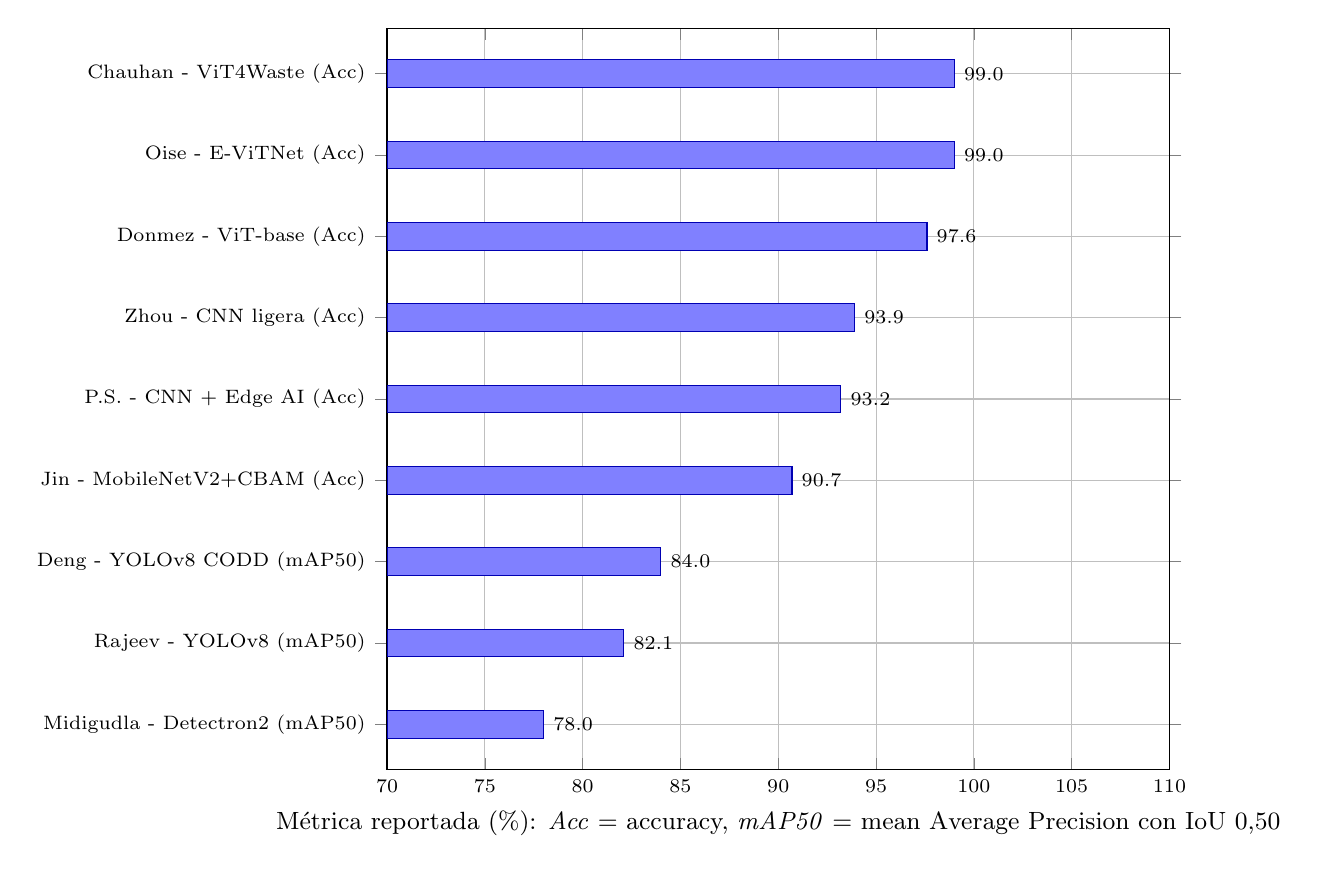
\begin{tikzpicture}
\begin{axis}[
    xbar,
    width=0.95\textwidth,
    height=11cm,
    xmin=70, xmax=110,
    xlabel={Métrica reportada (\%): \textit{Acc} = accuracy, \textit{mAP50} = mean Average Precision con IoU 0,50},
    ytick=data,
    yticklabels={
        Midigudla - Detectron2 (mAP50),
        Rajeev - YOLOv8 (mAP50),
        Deng - YOLOv8 CODD (mAP50),
        Jin - MobileNetV2+CBAM (Acc),
        P.S. - CNN + Edge AI (Acc),
        Zhou - CNN ligera (Acc),
        Donmez - ViT-base (Acc),
        Oise - E-ViTNet (Acc),
        Chauhan - ViT4Waste (Acc)
    },
    nodes near coords={
        \pgfmathprintnumber[fixed, fixed zerofill, precision=1]{\pgfplotspointmeta}
    },
    nodes near coords align={horizontal},
    bar width=10pt,
    enlarge y limits=0.07,
    grid=major,
    every node near coord/.append style={font=\scriptsize},
    label style={font=\small},
    tick label style={font=\scriptsize},
    legend style={at={(0.5,-0.18)}, anchor=north, legend columns=-1, font=\scriptsize}
]
\addplot[fill=blue!50, draw=blue!70!black] coordinates {
    (78.0, 1)
    (82.1, 2)
    (84.0, 3)
    (90.7, 4)
    (93.2, 5)
    (93.9, 6)
    (97.6, 7)
    (99.0, 8)
    (99.0, 9)
};
\end{axis}
\end{tikzpicture}
}
\caption{Análisis comparativo del rendimiento de los principales modelos de visión computacional aplicados a la clasificación y detección de residuos. Los valores corresponden a las métricas reportadas por cada autor sobre su conjunto de prueba; \textit{accuracy} y \textit{mAP50} no son directamente equivalentes y deben leerse como indicadores complementarios.}
\label{fig:comparativo_modelos}
\end{figure}
\subsection{Contexto regional y aplicado: gobernanza, normativa y realidades operativas}

La revisión muestra que la mayoría de los desarrollos de visión computacional aplicados a RAEE se han concentrado en China, India, Estados Unidos y la Unión Europea, mientras que la producción científica latinoamericana se centra en aspectos sociales, normativos y de gobernanza. \cite{jesiddiazbastosImpactoResiduosAparatos2025} ubican a Colombia como el cuarto generador de RAEE en América Latina y reportan que, a escala mundial, sólo cerca del 20\% de los 50 millones de toneladas anuales de RAEE se recicla adecuadamente; en la región, sólo el 3\% se gestiona formalmente, lo que se traduce en una pérdida estimada de 1\,700 millones de USD anuales. Estos autores confirman además la robustez del marco normativo colombiano (Ley 1672 de 2013, Decreto 284 de 2018, Política Nacional de Gestión Integral de RAEE de 2017 y Plan 2032) y describen la operación del Centro Nacional de Aprovechamiento de Residuos Electrónicos (Cenare), que ha retomado más de 206\,000 computadores.\\

\cite{zambranoyepezBuenasPracticasManejo2022} amplían esta lectura con un análisis comparativo de siete países latinoamericanos, evidenciando que México lidera la región en recuperación formal (36\%) y que en el caso colombiano programas como ``Computadores para Educar'' y ``Recicla tu móvil'' (646 toneladas, 907\,613 dispositivos) constituyen referentes regionales. \cite{clinckspoorAnalisisActoresInvolucrados2020}, en su estudio sobre Mar del Plata, introducen una caracterización útil para Colombia al diferenciar tres subsistemas operativos --formal, informal y \textit{extraformal}-- y al evidenciar el patrón regional de exportación de plaquetas a refinerías europeas, lo que se traduce en pérdida de valor agregado local. \cite{souzaCHALLENGESTRANSITIONCIRCULAR2025} confirma este patrón en Brasil mediante un análisis SODA con doce actores y agrega elementos adicionales como la tributación acumulativa y la presencia de importadores ``\textit{free riders}''.\\

En el caso colombiano, \cite{a.ceronRecyclableWasteClassification2025a} aporta el diagnóstico más cercano al problema de la tesis: Bogotá genera cerca de 7\,500 toneladas diarias de residuos, recupera menos del 20\% y cuenta con 26\,159 recicladores informales, mientras que las plantas distritales operan con clasificación principalmente manual y sin sensores espectrales o sistemas de visión computacional. La matriz SWOT incluida por el autor identifica como oportunidades específicas la incorporación de redes convolucionales entrenadas con datasets locales, IoT con contenedores inteligentes y blockchain para trazabilidad, lo que refuerza la pertinencia de la presente investigación. \cite{venegasmarcelModeloProcedimentalPara2020} añade un componente metodológico determinante: un modelo procedimental de cuatro indicadores (porcentaje masa por material, porcentaje masa por categoría, peligrosidad y reciclabilidad) que sirve de plantilla directa para construir el esquema de valoración económica de la presente propuesta.\\

El panorama brasileño se complementa con dos contribuciones que acercan aún más la mirada al objeto de la presente tesis. \cite{oliveiranetoCriticalBarriersMaterial2025}, en un estudio cualitativo aplicado a la cadena de RAEE en Brasil, identifican como barreras críticas la baja capacidad instalada de recuperación material, la dependencia de procesos manuales y la desconexión entre las etapas de identificación y comercialización; estos hallazgos guardan una similitud notable con el diagnóstico colombiano y refuerzan la pertinencia de articular clasificación visual y valoración económica desde un mismo sistema. \cite{oliveiranetoArtificialIntelligencebasedOptimization2025} avanzan en esa dirección al optimizar la cadena inversa de WEEE en São Paulo mediante técnicas de inteligencia artificial; su aporte más relevante para el presente trabajo es metodológico: muestran que el problema operativo se beneficia de combinar modelos predictivos con criterios económicos explícitos, un puente natural hacia el esquema de valoración propuesto. Por su parte, \cite{sharmaEnablersComputerVision2023} sistematizan los habilitadores que permiten que la visión computacional aterrice en plantas de e-waste --disponibilidad de datos representativos, integración con sistemas de gestión, alfabetización digital del personal y políticas públicas de soporte--, ofreciendo una lente que conecta la frontera tecnológica con la realidad organizacional.\\

A escala internacional, \cite{ottoniSustainabilityAssessmentBest2023} presentan una metodología SIG con once indicadores de sustentabilidad y cuatro logísticos para localizar plantas óptimas de procesamiento de PCB en Brasil; identifican ocho municipios candidatos --liderados por São Caetano do Sul, Jundiaí y Campinas-- con una capacidad potencial de aproximadamente 24 toneladas diarias. \cite{widanapathiranaElectricalElectronicWaste2023} confirman, desde el contexto sudasiático, que la informalidad domina entre el 60\% y el 90\% del tratamiento, y que el modelo de exportación de PCB a refinerías externas también se replica en India, Pakistán, Bangladesh y Sri Lanka. Por su parte, \cite{leeseHBM4EUEwasteStudy2025} aporta evidencia ocupacional crítica: en un estudio biomonitoring de ocho países europeos con 195 trabajadores, el plomo se mantiene como el contaminante de mayor preocupación con protección inadecuada, hallazgo extrapolable y especialmente relevante para los recicladores informales en Colombia. \cite{serpe20YearsEwaste2025} cierra el panorama regulatorio al sintetizar veinte años de regulación WEEE/RoHS en la Unión Europea, proyectar 82 Mt de RAEE para 2030 y advertir sobre un déficit económico de 40\,000 millones de USD si no se mejora la gestión global. \cite{guariniArtificialIntelligenceUrban2024} y \cite{bushuyevConceptualFrameworkSustainable2025} aportan, finalmente, los marcos de gobernanza inteligente que permiten integrar la clasificación automatizada en procesos urbanos más amplios.

\begin{table}[H]
\centering
\caption{Estudios con enfoque en contexto regional y normativo.}
\label{tab:matriz_regional}
\resizebox{\textwidth}{!}{%
\begin{tabular}{p{3.4cm}p{2.5cm}p{4cm}p{6cm}}
\hline
\textbf{Estudio} & \textbf{País / Región} & \textbf{Enfoque} & \textbf{Aporte clave para la tesis} \\
\hline
\cite{jesiddiazbastosImpactoResiduosAparatos2025} & Colombia / LAC & Diagnóstico ambiental y normativo & Marco legal colombiano y cifras de Cenare \\
\cite{zambranoyepezBuenasPracticasManejo2022} & LAC (7 países) & Buenas prácticas y normativa & Comparativa regional; lecciones de México y Chile \\
\cite{clinckspoorAnalisisActoresInvolucrados2020} & Argentina (Mar del Plata) & Actores y subsistemas & Tipología formal/informal/extraformal \\
\cite{a.ceronRecyclableWasteClassification2025a} & Colombia (Bogotá) & Diagnóstico + SWOT & Brechas de IA/CV en plantas distritales \\
\cite{venegasmarcelModeloProcedimentalPara2020} & Chile & Modelo procedimental RAEE & Plantilla de indicadores de valoración \\
\cite{souzaCHALLENGESTRANSITIONCIRCULAR2025} & Brasil & Cuellos de botella en EC & Tributación acumulativa e importadores ``free riders'' \\
\cite{ottoniSustainabilityAssessmentBest2023} & Brasil & SIG + sustentabilidad para PCB & Metodología extrapolable a Colombia \\
\cite{widanapathiranaElectricalElectronicWaste2023} & South Asia & Revisión sistemática & Patrón de informalidad y exportación \\
\cite{leeseHBM4EUEwasteStudy2025} & UE (8 países) & Biomonitoring ocupacional & Riesgos de exposición a Pb, Cd, Hg \\
\cite{serpe20YearsEwaste2025} & UE / Mundial & 20 años de regulación WEEE & Proyección 82 Mt y déficit USD 40\,000 M \\
\cite{guariniArtificialIntelligenceUrban2024} & UE & Decisiones urbanas con IA & Integración con gobernanza inteligente \\
\cite{bushuyevConceptualFrameworkSustainable2025} & UE & Framework BANI con IA & Caso aplicado de RAEE en universidad \\
\cite{oliveiranetoCriticalBarriersMaterial2025} & Brasil & Barreras a la recuperación de materiales & Diagnóstico cercano al caso colombiano \\
\cite{oliveiranetoArtificialIntelligencebasedOptimization2025} & Brasil (São Paulo) & Optimización con IA de la cadena WEEE & Articula IA con criterios económicos \\
\cite{sharmaEnablersComputerVision2023} & Mundial / aplicado & Habilitadores de visión computacional & Conecta CV con realidad organizacional \\
\hline
\end{tabular}}
\end{table}

\subsection{Gestión y valoración económica: sistemas de apoyo a la decisión y economía circular}

La tercera categoría agrupa los trabajos que articulan inteligencia artificial con sistemas de apoyo a la toma de decisiones (DSS) y con esquemas de valoración económica de los residuos. Las revisiones sistemáticas de \cite{janoClosingLoopSystematic2026} (147 artículos, 2019--2025) y \cite{dehabadi_how_2026} (335 artículos, 2015--2024) coinciden en señalar que el aprendizaje profundo concentra entre el 70\% y el 75\% de las aplicaciones de IA en gestión circular de RAEE y logística inversa, con CNN reportando precisiones del 95{,}88\% al 99\% y arquitecturas YOLO mAP50 entre 0{,}82 y 0{,}92. Ambos trabajos identifican brechas comunes: ausencia de \textit{datasets} estandarizados, fragmentación geográfica de los estudios, baja madurez de modelos federados y escasa adopción de IA generativa o LLMs en el dominio.\\

\cite{olawadeSmartWasteManagement2024}, en una revisión de 71 artículos, complementa este panorama mostrando cómo la integración de IoT, robótica colaborativa, visión computacional y \textit{blockchain} habilita un giro paradigmático del modelo lineal al circular. \cite{anithaSmartWasteEcosystems2025} avanzan un paso más al proponer un \textit{framework} de seis capas alineado con los principios de Industria 5.0, que combina \textit{Digital Twins}, \textit{Edge AI}, teoría de grafos y la jerarquía 9R, validado mediante simulación con resultados de --15\% a --20\% en frecuencia de recolección, --12\% a --18\% en consumo de combustible y aumentos de 25\% a 30\% en tasas de recuperación, con plásticos y RAEE liderando las ganancias. \cite{stephenSmartAIIoTBlockchain2026} consolida estas ideas en una arquitectura AI--IoT--\textit{blockchain} con \textit{just transition} validada en 142 sitios industriales, alcanzando un \textit{accuracy} de 95{,}0\%, un \textit{throughput} de 18\,t/h, una reducción del 34\% en consumo energético y un ROI del 22\% con período de retorno de 3{,}6 años a 2\,000\,t/día. Aunque el dominio es \textit{coal gangue}, su arquitectura es directamente trasladable a RAEE.\\

En el ámbito específico de la valoración, \cite{cespiLCAPreciousMetals2025} ofrece datos primarios de una refinería italiana que son fundamentales para la presente investigación: precios promedio en la década 2014--2024 de Au 60{,}5\,€/g, Ag 0{,}7\,€/g, Pt 27{,}2\,€/g, Pd 57{,}5\,€/g y Rh 205{,}0\,€/g, con huellas de carbono asociadas que oscilan entre 0{,}01 t\,CO\(_2\)/kg para la plata y 1{,}55 t\,CO\(_2\)/kg para el rodio. \cite{wangEwasteRecyclingIntegrated2025} aportan, desde una planta china, la composición típica de WPCB (Cu 16--20\%, Au 150--300\,ppm, Ag 600--1\,000\,ppm) y demuestran que escenarios optimizados de pirometalurgia logran recuperar hasta el 51{,}73\% de impactos ambientales con un período de retorno de 4{,}69 años. \cite{qinPreciousMetalRecycling2025} confirma la concentración 20--350 veces mayor de oro en placas de circuito impreso respecto a yacimientos primarios, y \cite{gheibiTurningEwasteValue2026} reporta un valor de recuperación específico de 73{,}1 USD/kg para Zn\(^{2+}\) desde baterías alcalinas. \cite{mtibeSustainableValorizationConversion2023} aportan que los plásticos representan cerca del 15\% del peso de los RAEE, mayoritariamente con destino a relleno sanitario, y demuestran que filamentos 3D de policarbonato reciclado alcanzan el 83\% de la resistencia del ABS virgen con una reducción del 28\% en emisiones de CO\(_2\).\\

Los enfoques específicos de logística inversa y diseño de redes consolidan estos hallazgos a través de diversas aplicaciones recientes. \cite{almuwalladManagingEwasteReverse2026} extiende el modelo a baterías Li-ion en Arabia Saudita combinando MILP, optimización neutrosófica y cadenas de Markov para fallas. \cite{rahmanDecisionSupportTool2023} introduce el algoritmo bio-inspirado HACO en una herramienta de soporte a la decisión que reduce el costo de procesamiento de 0{,}11 a 0{,}07 USD/lb. \cite{alzubiBridgingCircularityMeasurement2025} y \cite{alsabtOptimizingWasteManagement2024} aportan herramientas de medición de circularidad y predicción global de generación, con XGBoost alcanzando un \(R^2\) de 0{,}908. \cite{banyaiRealTimeOperationalDecision2025} muestra cómo la integración de IoT y \textit{cloud computing} permite optimización en tiempo real, con una reducción del 12{,}2\% en costos de recolección municipal.\\

Las revisiones sistemáticas de \cite{leeEnvironmentalEconomicImpacts2024b} (159 estudios) y \cite{elgarahyRevitalizingCircularEconomy2024} aportan una conclusión sobria: no existe consenso sobre la viabilidad económica del reciclaje formal de RAEE, y los estudios actuales presentan vacíos metodológicos significativos al separar el análisis ambiental del análisis económico. \cite{dixitBiologicalApproachesEwaste2023} cuantifica que el reciclaje formal de RAEE representó cerca de 57\,000 millones de USD en valor recuperado y 681\,000 empleos en el sector estadounidense entre 2012 y 2020, lo cual marca un orden de magnitud útil para evaluar el potencial colombiano. \cite{heDrivingSustainableCircular2024} consolida esta lectura desde el ángulo del análisis de ciclo de vida (LCA): muestra que la verdadera ganancia ambiental del reciclaje de RAEE depende menos de la pureza del flujo recuperado y más del nivel de circularidad alcanzado al cierre del proceso, lo cual refuerza la idea de pasar del simple reciclaje al \textit{upcycling}. Esa misma transición es desarrollada por \cite{dagwar_upcycling_2026}, quienes documentan cómo el rediseño de productos a partir de RAEE permite generar materiales funcionales con menor toxicidad y un costo ambiental inferior al de las materias primas vírgenes, perspectiva que añade una dimensión adicional al esquema de valoración económica que se construirá en este proyecto.\\

En el plano metodológico, \cite{seikhIdentifyingSustainableStrategies2024} desarrollan un esquema de toma de decisiones grupal basado en confianza para evaluar estrategias sostenibles de gestión de RAEE; el aporte resulta especialmente útil para esta investigación porque ofrece una manera transparente de combinar criterios técnicos, económicos y sociales dentro de una única función de decisión, problema que aparece de forma recurrente cuando se intenta articular clasificación visual y valoración económica. Finalmente, \cite{varshaDataDrivenEWasteManagement2025a} muestran que algoritmos clásicos de \textit{machine learning} pueden mejorar la planeación de la recolección y el reciclaje cuando se entrenan sobre datos heterogéneos del propio sistema; este resultado valida un principio que se asume en el presente trabajo: las decisiones operativas se benefician de un soporte cuantitativo continuo, incluso antes de incorporar arquitecturas profundas más sofisticadas.

\begin{table}[H]
\centering
\caption{Estudios con enfoque en gestión y valoración económica.}
\label{tab:matriz_gestion}
\resizebox{\textwidth}{!}{%
\begin{tabular}{p{3.4cm}p{3.5cm}p{3.5cm}p{5cm}}
\hline
\textbf{Estudio} & \textbf{Tipo de aporte} & \textbf{Métodos / técnicas} & \textbf{Cifras clave} \\
\hline
\cite{janoClosingLoopSystematic2026} & Revisión sistemática & DL/ML en EC & 147 art.; CNN 95{,}88--99\% \\
\cite{dehabadi_how_2026} & Revisión sistemática & IA en logística inversa & 335 art.; metaheurísticas 74\% \\
\cite{olawadeSmartWasteManagement2024} & Revisión & IA + IoT + robótica & CNN 93\%; 71 art. \\
\cite{anithaSmartWasteEcosystems2025} & Framework Industria 5.0 & DT + Edge-AI + 9R & --15--20\% recolección \\
\cite{stephenSmartAIIoTBlockchain2026} & Arquitectura integrada & AI--IoT--Blockchain & Acc 95\%; ROI 22\% \\
\cite{cespiLCAPreciousMetals2025} & LCA y precios & Datos primarios refinería & Au 60{,}5 €/g; Ag 0{,}7 €/g \\
\cite{wangEwasteRecyclingIntegrated2025} & LCA + TEA & Pirometalurgia WPCB & Cu 16--20\%; payback 4{,}69 a \\
\cite{qinPreciousMetalRecycling2025} & Bibliometría & Recuperación de PGM & Au 200--350 g/t en PCB \\
\cite{gheibiTurningEwasteValue2026} & Experimental & LDC + RSM + ANN & Zn 73{,}1 USD/kg \\
\cite{mtibeSustainableValorizationConversion2023} & Revisión & Reciclaje de plásticos & Filamentos PC: 83\% resistencia ABS \\
\cite{almuwalladManagingEwasteReverse2026} & MILP + neutrosófico & EV + Li-ion KSA & 595 kt; pyro/hydro/direct \\
\cite{rahmanDecisionSupportTool2023} & DSS bio-inspirado & HACO + DES & --36\% costo unitario \\
\cite{alzubiBridgingCircularityMeasurement2025} & System Dynamics & Bibliometría + SD & --160 Mt CO\(_2\); +0{,}01 empleos/t \\
\cite{alsabtOptimizingWasteManagement2024} & XGBoost + LP & Predicción global & 85\% precisión; \(R^2\)=0{,}908 \\
\cite{banyaiRealTimeOperationalDecision2025} & IoT + cloud + ML & Ruteo en tiempo real & --12{,}2\% costo \\
\cite{leeEnvironmentalEconomicImpacts2024b} & Revisión sistemática & 159 estudios & Sin consenso económico \\
\cite{elgarahyRevitalizingCircularEconomy2024} & Revisión & Mecánico/químico/ biológico & 60\% metales; 15\% plásticos \\
\cite{dixitBiologicalApproachesEwaste2023} & Revisión + valor & Biolixiviación & 57\,000 M USD; 681\,000 empleos \\
\cite{heDrivingSustainableCircular2024} & Revisión LCA & Ciclo de vida e-waste & Circularidad > pureza \\
\cite{dagwar_upcycling_2026} & Upcycling RAEE & Materiales funcionales & Menor toxicidad y CO\(_2\) \\
\cite{seikhIdentifyingSustainableStrategies2024} & Decisión grupal & Confidence-based DM & Integra criterios técnicos, econ.\ y sociales \\
\cite{varshaDataDrivenEWasteManagement2025a} & ML clásico aplicado & Datos heterogéneos del sistema & Mejora planeación de recolección \\
\hline
\end{tabular}}
\end{table}

% ======================================================================
\subsection{Despliegue en hardware de bajo costo: \textit{edge AI} para clasificación de residuos}
La cuarta categoría reúne los estudios que responden de manera directa a la pregunta P4, al implementar y medir modelos de visión computacional sobre plataformas de cómputo asequibles. En el escenario de sólo CPU, \cite{castrobelloConvolutionalNeuralNetwork2025} entrenaron YOLOv4-tiny, YOLOv7-tiny, YOLOv8-nano y YOLOv9-tiny sobre un conjunto propio de 1\,883 imágenes de residuos orgánicos e inorgánicos y los compararon en una Raspberry Pi 4 Model B en términos de precisión, velocidad de inferencia y uso de recursos; YOLOv8-nano alcanzó un mAP50 de 0{,}976 con un tiempo de inferencia cercano a 1{,}5\,s por imagen, mientras que el uso de CPU osciló entre el 80\% y el 97\%, lo que evidencia que el procesador es el recurso crítico en esta configuración. \cite{daoDesignImplementationRealTime2026} compararon YOLOv5n, YOLOv7-tiny y YOLOv8n bajo las mismas condiciones e integraron el mejor modelo con un controlador y un actuador de separación; YOLOv8n obtuvo un mAP50 de 0{,}888, una \textit{precision} de 0{,}847 y un \textit{recall} de 0{,}805, con una latencia de 150\,ms ($\sim$6{,}7\,FPS) en la CPU de una Raspberry Pi 5. De forma similar, \cite{yulizaRaspberryPi4Ultrasonic2024} implementaron una CNN en una Raspberry Pi 4 para cuatro categorías de residuos (plástico, metal, peligrosos y orgánicos), con un \textit{accuracy} del 90\% y monitoreo IoT del nivel de llenado.\\

La incorporación de aceleradores neuronales de bajo costo reduce de forma significativa la latencia. \cite{mutarAIBasedModelHome2026} optimizaron YOLOv5s para la NPU del Raspberry Pi 5 AI Kit y clasificaron cinco categorías de residuos domésticos con un \textit{accuracy} del 95{,}2\%, una latencia de 45\,ms por imagen y un consumo promedio de 5{,}2\,W. Este resultado es coherente con el de \cite{p.sLowPowerEdgeAI2026}, único trabajo de este grupo aplicado específicamente a RAEE, que emplea la misma familia de aceleradores (Hailo-8L) con un consumo de 7{,}8\,W.\\

Los estudios de \textit{benchmarking} aportan los criterios para seleccionar el dispositivo y la técnica de optimización. \cite{zagitovComparativeAnalysisNeural2024} compararon MobileNetV2-SSD, CenterNet, EfficientDet, YOLOv5, YOLOv7, YOLOv7-Tiny y YOLOv8 en Raspberry Pi 3B, Raspberry Pi 4B y Jetson Nano con TensorFlow Lite, aplicando cuantización posterior al entrenamiento (PTQ) y cuantización consciente del entrenamiento (QAT), y concluyeron que la elección del algoritmo depende de los requisitos de la tarea. \cite{alqahtaniBenchmarkingDeepLearning2024} evaluaron YOLOv8 (n, s, m), EfficientDet-Lite y SSD en Raspberry Pi 3, 4 y 5, con y sin acelerador Coral Edge TPU, y en Jetson Orin Nano, midiendo consumo energético, tiempo de inferencia y mAP; el Jetson Orin Nano resultó la opción más rápida y eficiente en energía, aunque con el mayor consumo en reposo. \cite{magalhaesBenchmarkingEdgeComputing2023}, por su parte, mostraron que la TPU y la GPU embebida son las plataformas más eficientes energéticamente, con consumos cercanos a 5\,W. En conjunto, estos trabajos confirman que una Raspberry Pi 5, con o sin acelerador, constituye una plataforma adecuada para el prototipo, y que la cuantización es la técnica de optimización determinante para su despliegue.

\begin{center}
\captionof{table}{Estudios sobre despliegue de visión computacional en hardware de bajo costo.}
\label{tab:matriz_edge}
\resizebox{\textwidth}{!}{%
\begin{tabular}{p{3.2cm}p{3.4cm}p{3.4cm}p{2.4cm}p{4.6cm}}
\hline
\textbf{Estudio} & \textbf{Hardware} & \textbf{Modelo(s)} & \textbf{Dominio} & \textbf{Resultados clave} \\
\hline
\cite{castrobelloConvolutionalNeuralNetwork2025} & Raspberry Pi 4B (CPU) & YOLOv4-tiny, v7-tiny, v8-nano, v9-tiny & Residuos sólidos & YOLOv8-nano mAP50 0{,}976; $\sim$1{,}5\,s/img; CPU 80--97\% \\
\cite{daoDesignImplementationRealTime2026} & Raspberry Pi 5 (CPU) & YOLOv5n, v7-tiny, v8n & Residuos + actuador & YOLOv8n mAP50 0{,}888; 150\,ms; 6{,}7\,FPS \\
\cite{yulizaRaspberryPi4Ultrasonic2024} & Raspberry Pi 4 (CPU) & CNN & Residuos (4 clases) & Acc 90\%; monitoreo IoT \\
\cite{mutarAIBasedModelHome2026} & Raspberry Pi 5 + AI Kit (NPU) & YOLOv5s & Residuos domésticos & Acc 95{,}2\%; 45\,ms; 5{,}2\,W \\
\cite{p.sLowPowerEdgeAI2026} & Raspberry Pi + Hailo-8L & CNN + fusión multisensor & RAEE & Acc 93{,}2\%; 7{,}8\,W \\
\cite{zagitovComparativeAnalysisNeural2024} & RPi 3B, RPi 4B, Jetson Nano & SSD, EfficientDet, YOLOv5/v7/v8 & Benchmark & Comparación con PTQ y QAT en TFLite \\
\cite{alqahtaniBenchmarkingDeepLearning2024} & RPi 3/4/5, Coral TPU, Jetson Orin Nano & YOLOv8 n/s/m, EfficientDet-Lite, SSD & Benchmark & Energía, latencia y mAP por dispositivo \\
\cite{magalhaesBenchmarkingEdgeComputing2023} & Jetson Nano/TX2, Coral, Xilinx & SSD & Benchmark (agrícola) & TPU y GPU embebida $\sim$5\,W \\
\hline
\end{tabular}}
\end{center}

\section{Brechas de Investigación Identificadas}

El análisis transversal de los 58 estudios permite responder a las preguntas de investigación formuladas. Respecto a P1, las arquitecturas dominantes son CNN ligeras orientadas a \textit{edge}, detectores tipo YOLO (con YOLOv8 como referencia operativa) y \textit{Vision Transformers} en la frontera más reciente, con métricas reportadas entre 90\% y 99\% de \textit{accuracy} y entre 0{,}82 y 0{,}92 de mAP50. En cuanto a P2, los datasets utilizados son mayoritariamente propietarios y de tamaño limitado (entre 164 y 14\,683 imágenes), con el problema reiterado de la ausencia de \textit{datasets} públicos específicos para RAEE en contextos latinoamericanos. Con relación a P3, sólo un subconjunto reducido de trabajos integra explícitamente la clasificación visual con esquemas de valoración económica o sistemas de apoyo a la decisión \cite{joshiSustainableEWasteManagement2024,obayemiAutomatedWEEESortation2025a,stephenSmartAIIoTBlockchain2026,p.sLowPowerEdgeAI2026}, y la mayoría se concentra en optimización logística sin una capa visual estandarizada. En relación con P4, los desarrollos más recientes muestran que la combinación de cuantización, NPUs especializadas y fusión multisensorial permite operar por debajo de los 10\,W con latencias inferiores a 5\,s, lo que vuelve viable el despliegue en escenarios con conectividad limitada; la búsqueda complementaria confirma que detectores ligeros como YOLOv8n pueden ejecutarse en una Raspberry Pi 5 con latencias de 150\,ms en CPU y de 45\,ms con acelerador neuronal \cite{daoDesignImplementationRealTime2026,mutarAIBasedModelHome2026}, aunque casi siempre sobre residuos sólidos municipales y no sobre componentes de RAEE. Finalmente, frente a P5, se confirma que el contexto colombiano sólo aparece de manera parcial en \cite{a.ceronRecyclableWasteClassification2025a} y \cite{jesiddiazbastosImpactoResiduosAparatos2025}, y que ninguno de los estudios analizados implementa modelos de visión computacional entrenados sobre datasets locales de RAEE.\\

A partir de este balance se identifican seis brechas principales que justifican la presente investigación:

\begin{enumerate}
    \item \textbf{Ausencia de datasets locales}: ninguno de los estudios revisados utiliza imágenes de RAEE capturadas en el contexto colombiano, lo que limita la transferibilidad directa de los modelos del estado del arte y demanda la curaduría de un conjunto propio.
    \item \textbf{Desconexión entre clasificación y valoración}: la mayoría de las propuestas operan en silos, sin integrar de forma sistemática el resultado de la clasificación con un esquema de estimación del potencial económico o de aprovechamiento del residuo \cite{simaeiAIbasedDecisionSupport2024,anandhMultiobjectiveMetaheuristicsOptimize2024}.
    \item \textbf{Brechas tecnológicas en plantas regionales}: las plantas distritales en Bogotá y otras ciudades de América Latina operan con clasificación predominantemente manual y sin sensores espectrales, condición que confirma el espacio para soluciones \textit{edge} y de bajo costo \cite{a.ceronRecyclableWasteClassification2025a, clinckspoorAnalisisActoresInvolucrados2020}.
    \item \textbf{Limitada incorporación del sector informal y de la realidad ocupacional}: los modelos de logística inversa y los frameworks de IA suelen ignorar la informalidad y los riesgos de exposición ocupacional documentados por \cite{leeseHBM4EUEwasteStudy2025} y \cite{widanapathiranaElectricalElectronicWaste2023}.
    \item \textbf{Falta de consenso sobre la viabilidad económica}: las revisiones sistemáticas \cite{leeEnvironmentalEconomicImpacts2024b, janoClosingLoopSystematic2026} subrayan que la literatura aún no cuenta con metodologías que integren impactos ambientales, económicos y sociales de manera coherente para RAEE, una brecha que la presente propuesta busca atender mediante la combinación de un modelo de visión computacional con un esquema de valoración económica adaptado al contexto colombiano.
    \item \textbf{Escasa validación de clasificadores de RAEE en hardware de bajo costo}: los trabajos que despliegan modelos en Raspberry Pi o en aceleradores neuronales de bajo consumo se concentran en residuos sólidos municipales \cite{castrobelloConvolutionalNeuralNetwork2025,daoDesignImplementationRealTime2026,mutarAIBasedModelHome2026}, y sólo \cite{p.sLowPowerEdgeAI2026} e \cite{ilievEmbeddedSystemEwaste2023} lo hacen con RAEE; no existe, por tanto, evidencia sistemática del desempeño de clasificadores de componentes de RAEE bajo las restricciones de cómputo, memoria y energía de estas plataformas.
\end{enumerate}

En conjunto, el estado del arte confirma que existen los componentes tecnológicos necesarios para construir un sistema de apoyo a la toma de decisiones basado en visión computacional y valoración económica para la gestión de RAEE, pero que su integración bajo las condiciones operativas colombianas y con un nivel de granularidad adecuado al tipo de objeto sigue siendo una oportunidad de investigación abierta.\\

Esta lectura sostiene de forma directa los cinco objetivos específicos del proyecto. La primera brecha legitima la decisión de \emph{diseñar un modelo de visión computacional con \textit{transfer learning}} (objetivo 1), apoyado en arquitecturas que ya han demostrado solvencia en la literatura. La segunda y la quinta brecha justifican la formulación de un \emph{esquema de valoración económica} alineado con la clasificación visual (objetivo 2), apoyado en los datos primarios de \cite{cespiLCAPreciousMetals2025}, \cite{wangEwasteRecyclingIntegrated2025} y \cite{qinPreciousMetalRecycling2025}, así como en los marcos de decisión propuestos por \cite{seikhIdentifyingSustainableStrategies2024} y \cite{venegasmarcelModeloProcedimentalPara2020}. La sexta brecha fundamenta la \emph{implementación y optimización del modelo en hardware de bajo costo} (objetivo 3), siguiendo las prácticas de cuantización y evaluación de \cite{zagitovComparativeAnalysisNeural2024} y \cite{alqahtaniBenchmarkingDeepLearning2024}. La tercera brecha respalda la integración de ambos componentes en un \emph{prototipo} pensado para condiciones reales de plantas colombianas (objetivo 4), reforzada por las experiencias de \cite{a.ceronRecyclableWasteClassification2025a}, \cite{ilievEmbeddedSystemEwaste2023} y \cite{p.sLowPowerEdgeAI2026}. Por último, el análisis comparativo de modelos presentado en la Figura \ref{fig:comparativo_modelos} y en la Tabla \ref{tab:matriz_edge} ofrece una línea base concreta para la \emph{evaluación frente al proceso manual} prevista en el objetivo 5. Este encaje entre brechas y objetivos confirma además la pertinencia de la justificación y del planteamiento del problema, en particular en lo relativo al cuello de botella manual descrito por \cite{a.ceronRecyclableWasteClassification2025a} y al diagnóstico colombiano de \cite{jesiddiazbastosImpactoResiduosAparatos2025}.
